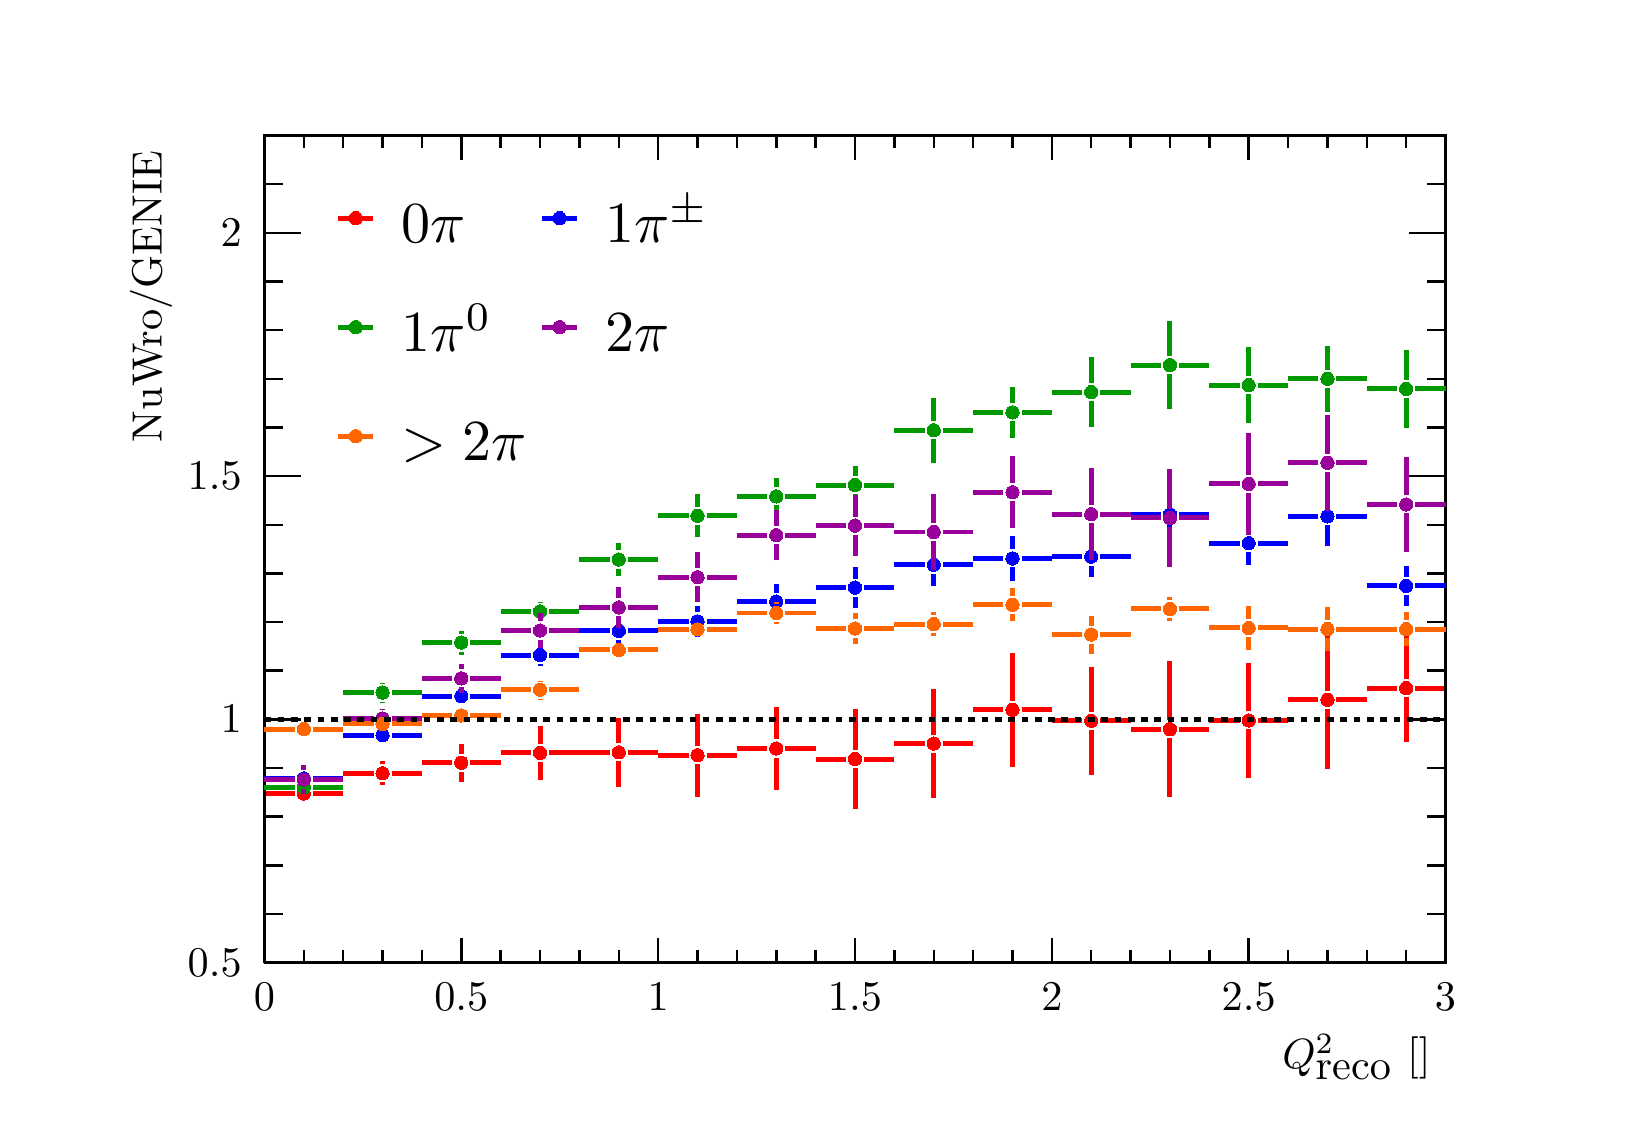
\begin{tikzpicture}
\pgfdeclareplotmark{cross} {
\pgfpathmoveto{\pgfpoint{-0.3\pgfplotmarksize}{\pgfplotmarksize}}
\pgfpathlineto{\pgfpoint{+0.3\pgfplotmarksize}{\pgfplotmarksize}}
\pgfpathlineto{\pgfpoint{+0.3\pgfplotmarksize}{0.3\pgfplotmarksize}}
\pgfpathlineto{\pgfpoint{+1\pgfplotmarksize}{0.3\pgfplotmarksize}}
\pgfpathlineto{\pgfpoint{+1\pgfplotmarksize}{-0.3\pgfplotmarksize}}
\pgfpathlineto{\pgfpoint{+0.3\pgfplotmarksize}{-0.3\pgfplotmarksize}}
\pgfpathlineto{\pgfpoint{+0.3\pgfplotmarksize}{-1.\pgfplotmarksize}}
\pgfpathlineto{\pgfpoint{-0.3\pgfplotmarksize}{-1.\pgfplotmarksize}}
\pgfpathlineto{\pgfpoint{-0.3\pgfplotmarksize}{-0.3\pgfplotmarksize}}
\pgfpathlineto{\pgfpoint{-1.\pgfplotmarksize}{-0.3\pgfplotmarksize}}
\pgfpathlineto{\pgfpoint{-1.\pgfplotmarksize}{0.3\pgfplotmarksize}}
\pgfpathlineto{\pgfpoint{-0.3\pgfplotmarksize}{0.3\pgfplotmarksize}}
\pgfpathclose
\pgfusepathqstroke
}
\pgfdeclareplotmark{cross*} {
\pgfpathmoveto{\pgfpoint{-0.3\pgfplotmarksize}{\pgfplotmarksize}}
\pgfpathlineto{\pgfpoint{+0.3\pgfplotmarksize}{\pgfplotmarksize}}
\pgfpathlineto{\pgfpoint{+0.3\pgfplotmarksize}{0.3\pgfplotmarksize}}
\pgfpathlineto{\pgfpoint{+1\pgfplotmarksize}{0.3\pgfplotmarksize}}
\pgfpathlineto{\pgfpoint{+1\pgfplotmarksize}{-0.3\pgfplotmarksize}}
\pgfpathlineto{\pgfpoint{+0.3\pgfplotmarksize}{-0.3\pgfplotmarksize}}
\pgfpathlineto{\pgfpoint{+0.3\pgfplotmarksize}{-1.\pgfplotmarksize}}
\pgfpathlineto{\pgfpoint{-0.3\pgfplotmarksize}{-1.\pgfplotmarksize}}
\pgfpathlineto{\pgfpoint{-0.3\pgfplotmarksize}{-0.3\pgfplotmarksize}}
\pgfpathlineto{\pgfpoint{-1.\pgfplotmarksize}{-0.3\pgfplotmarksize}}
\pgfpathlineto{\pgfpoint{-1.\pgfplotmarksize}{0.3\pgfplotmarksize}}
\pgfpathlineto{\pgfpoint{-0.3\pgfplotmarksize}{0.3\pgfplotmarksize}}
\pgfpathclose
\pgfusepathqfillstroke
}
\pgfdeclareplotmark{newstar} {
\pgfpathmoveto{\pgfqpoint{0pt}{\pgfplotmarksize}}
\pgfpathlineto{\pgfqpointpolar{44}{0.5\pgfplotmarksize}}
\pgfpathlineto{\pgfqpointpolar{18}{\pgfplotmarksize}}
\pgfpathlineto{\pgfqpointpolar{-20}{0.5\pgfplotmarksize}}
\pgfpathlineto{\pgfqpointpolar{-54}{\pgfplotmarksize}}
\pgfpathlineto{\pgfqpointpolar{-90}{0.5\pgfplotmarksize}}
\pgfpathlineto{\pgfqpointpolar{234}{\pgfplotmarksize}}
\pgfpathlineto{\pgfqpointpolar{198}{0.5\pgfplotmarksize}}
\pgfpathlineto{\pgfqpointpolar{162}{\pgfplotmarksize}}
\pgfpathlineto{\pgfqpointpolar{134}{0.5\pgfplotmarksize}}
\pgfpathclose
\pgfusepathqstroke
}
\pgfdeclareplotmark{newstar*} {
\pgfpathmoveto{\pgfqpoint{0pt}{\pgfplotmarksize}}
\pgfpathlineto{\pgfqpointpolar{44}{0.5\pgfplotmarksize}}
\pgfpathlineto{\pgfqpointpolar{18}{\pgfplotmarksize}}
\pgfpathlineto{\pgfqpointpolar{-20}{0.5\pgfplotmarksize}}
\pgfpathlineto{\pgfqpointpolar{-54}{\pgfplotmarksize}}
\pgfpathlineto{\pgfqpointpolar{-90}{0.5\pgfplotmarksize}}
\pgfpathlineto{\pgfqpointpolar{234}{\pgfplotmarksize}}
\pgfpathlineto{\pgfqpointpolar{198}{0.5\pgfplotmarksize}}
\pgfpathlineto{\pgfqpointpolar{162}{\pgfplotmarksize}}
\pgfpathlineto{\pgfqpointpolar{134}{0.5\pgfplotmarksize}}
\pgfpathclose
\pgfusepathqfillstroke
}
\definecolor{c}{rgb}{1,1,1};
\draw [color=c, fill=c] (0,0) rectangle (20,13.639);
\draw [color=c, fill=c] (3,1.77307) rectangle (18,12.2751);
\definecolor{c}{rgb}{0,0,0};
\draw [c,line width=0.9] (3,1.77307) -- (3,12.2751) -- (18,12.2751) -- (18,1.77307) -- (3,1.77307);
\definecolor{c}{rgb}{1,1,1};
\draw [color=c, fill=c] (3,1.77307) rectangle (18,12.2751);
\definecolor{c}{rgb}{0,0,0};
\draw [c,line width=0.9] (3,1.77307) -- (3,12.2751) -- (18,12.2751) -- (18,1.77307) -- (3,1.77307);
\definecolor{c}{rgb}{1,0,0};
\draw [c,line width=1.8] (3,3.91911) -- (3.38539,3.91911);
\draw [c,line width=1.8] (3.61461,3.91911) -- (4,3.91911);
\foreach \P in {(3.5,3.91911)}{\draw[mark options={color=c,fill=c},mark size=2.402402pt, line width=0.000000pt, mark=*] plot coordinates {\P};}
\draw [c,line width=1.8] (4.5,4.02491) -- (4.5,4.06197);
\draw [c,line width=1.8] (4.5,4.2912) -- (4.5,4.32827);
\draw [c,line width=1.8] (4,4.17659) -- (4.38539,4.17659);
\draw [c,line width=1.8] (4.61461,4.17659) -- (5,4.17659);
\foreach \P in {(4.5,4.17659)}{\draw[mark options={color=c,fill=c},mark size=2.402402pt, line width=0.000000pt, mark=*] plot coordinates {\P};}
\draw [c,line width=1.8] (5.5,4.06967) -- (5.5,4.19653);
\draw [c,line width=1.8] (5.5,4.42576) -- (5.5,4.55262);
\draw [c,line width=1.8] (5,4.31115) -- (5.38539,4.31115);
\draw [c,line width=1.8] (5.61461,4.31115) -- (6,4.31115);
\foreach \P in {(5.5,4.31115)}{\draw[mark options={color=c,fill=c},mark size=2.402402pt, line width=0.000000pt, mark=*] plot coordinates {\P};}
\draw [c,line width=1.8] (6.5,4.09054) -- (6.5,4.32215);
\draw [c,line width=1.8] (6.5,4.55138) -- (6.5,4.78299);
\draw [c,line width=1.8] (6,4.43676) -- (6.38539,4.43676);
\draw [c,line width=1.8] (6.61461,4.43676) -- (7,4.43676);
\foreach \P in {(6.5,4.43676)}{\draw[mark options={color=c,fill=c},mark size=2.402402pt, line width=0.000000pt, mark=*] plot coordinates {\P};}
\draw [c,line width=1.8] (7.5,4.00439) -- (7.5,4.32806);
\draw [c,line width=1.8] (7.5,4.55729) -- (7.5,4.88095);
\draw [c,line width=1.8] (7,4.44267) -- (7.38539,4.44267);
\draw [c,line width=1.8] (7.61461,4.44267) -- (8,4.44267);
\foreach \P in {(7.5,4.44267)}{\draw[mark options={color=c,fill=c},mark size=2.402402pt, line width=0.000000pt, mark=*] plot coordinates {\P};}
\draw [c,line width=1.8] (8.5,3.88168) -- (8.5,4.2921);
\draw [c,line width=1.8] (8.5,4.52133) -- (8.5,4.93175);
\draw [c,line width=1.8] (8,4.40671) -- (8.38539,4.40671);
\draw [c,line width=1.8] (8.61461,4.40671) -- (9,4.40671);
\foreach \P in {(8.5,4.40671)}{\draw[mark options={color=c,fill=c},mark size=2.402402pt, line width=0.000000pt, mark=*] plot coordinates {\P};}
\draw [c,line width=1.8] (9.5,3.95924) -- (9.5,4.37703);
\draw [c,line width=1.8] (9.5,4.60626) -- (9.5,5.02405);
\draw [c,line width=1.8] (9,4.49165) -- (9.38539,4.49165);
\draw [c,line width=1.8] (9.61461,4.49165) -- (10,4.49165);
\foreach \P in {(9.5,4.49165)}{\draw[mark options={color=c,fill=c},mark size=2.402402pt, line width=0.000000pt, mark=*] plot coordinates {\P};}
\draw [c,line width=1.8] (10.5,3.72077) -- (10.5,4.24284);
\draw [c,line width=1.8] (10.5,4.47207) -- (10.5,4.99414);
\draw [c,line width=1.8] (10,4.35746) -- (10.3854,4.35746);
\draw [c,line width=1.8] (10.6146,4.35746) -- (11,4.35746);
\foreach \P in {(10.5,4.35746)}{\draw[mark options={color=c,fill=c},mark size=2.402402pt, line width=0.000000pt, mark=*] plot coordinates {\P};}
\draw [c,line width=1.8] (11.5,3.86667) -- (11.5,4.43937);
\draw [c,line width=1.8] (11.5,4.6686) -- (11.5,5.24131);
\draw [c,line width=1.8] (11,4.55399) -- (11.3854,4.55399);
\draw [c,line width=1.8] (11.6146,4.55399) -- (12,4.55399);
\foreach \P in {(11.5,4.55399)}{\draw[mark options={color=c,fill=c},mark size=2.402402pt, line width=0.000000pt, mark=*] plot coordinates {\P};}
\draw [c,line width=1.8] (12.5,4.26285) -- (12.5,4.86913);
\draw [c,line width=1.8] (12.5,5.09835) -- (12.5,5.70464);
\draw [c,line width=1.8] (12,4.98374) -- (12.3854,4.98374);
\draw [c,line width=1.8] (12.6146,4.98374) -- (13,4.98374);
\foreach \P in {(12.5,4.98374)}{\draw[mark options={color=c,fill=c},mark size=2.402402pt, line width=0.000000pt, mark=*] plot coordinates {\P};}
\draw [c,line width=1.8] (13.5,4.16025) -- (13.5,4.72872);
\draw [c,line width=1.8] (13.5,4.95794) -- (13.5,5.52641);
\draw [c,line width=1.8] (13,4.84333) -- (13.3854,4.84333);
\draw [c,line width=1.8] (13.6146,4.84333) -- (14,4.84333);
\foreach \P in {(13.5,4.84333)}{\draw[mark options={color=c,fill=c},mark size=2.402402pt, line width=0.000000pt, mark=*] plot coordinates {\P};}
\draw [c,line width=1.8] (14.5,3.87445) -- (14.5,4.62216);
\draw [c,line width=1.8] (14.5,4.85139) -- (14.5,5.59911);
\draw [c,line width=1.8] (14,4.73678) -- (14.3854,4.73678);
\draw [c,line width=1.8] (14.6146,4.73678) -- (15,4.73678);
\foreach \P in {(14.5,4.73678)}{\draw[mark options={color=c,fill=c},mark size=2.402402pt, line width=0.000000pt, mark=*] plot coordinates {\P};}
\draw [c,line width=1.8] (15.5,4.12242) -- (15.5,4.73293);
\draw [c,line width=1.8] (15.5,4.96216) -- (15.5,5.57267);
\draw [c,line width=1.8] (15,4.84755) -- (15.3854,4.84755);
\draw [c,line width=1.8] (15.6146,4.84755) -- (16,4.84755);
\foreach \P in {(15.5,4.84755)}{\draw[mark options={color=c,fill=c},mark size=2.402402pt, line width=0.000000pt, mark=*] plot coordinates {\P};}
\draw [c,line width=1.8] (16.5,4.23132) -- (16.5,4.99592);
\draw [c,line width=1.8] (16.5,5.22515) -- (16.5,5.98976);
\draw [c,line width=1.8] (16,5.11054) -- (16.3854,5.11054);
\draw [c,line width=1.8] (16.6146,5.11054) -- (17,5.11054);
\foreach \P in {(16.5,5.11054)}{\draw[mark options={color=c,fill=c},mark size=2.402402pt, line width=0.000000pt, mark=*] plot coordinates {\P};}
\draw [c,line width=1.8] (17.5,4.57864) -- (17.5,5.14441);
\draw [c,line width=1.8] (17.5,5.37364) -- (17.5,5.93942);
\draw [c,line width=1.8] (17,5.25903) -- (17.3854,5.25903);
\draw [c,line width=1.8] (17.6146,5.25903) -- (18,5.25903);
\foreach \P in {(17.5,5.25903)}{\draw[mark options={color=c,fill=c},mark size=2.402402pt, line width=0.000000pt, mark=*] plot coordinates {\P};}
\definecolor{c}{rgb}{0,0,0};
\draw [c,line width=0.9] (3,1.77307) -- (18,1.77307);
\draw [c,line width=0.9] (3,2.07994) -- (3,1.77307);
\draw [c,line width=0.9] (3.5,1.9265) -- (3.5,1.77307);
\draw [c,line width=0.9] (4,1.9265) -- (4,1.77307);
\draw [c,line width=0.9] (4.5,1.9265) -- (4.5,1.77307);
\draw [c,line width=0.9] (5,1.9265) -- (5,1.77307);
\draw [c,line width=0.9] (5.5,2.07994) -- (5.5,1.77307);
\draw [c,line width=0.9] (6,1.9265) -- (6,1.77307);
\draw [c,line width=0.9] (6.5,1.9265) -- (6.5,1.77307);
\draw [c,line width=0.9] (7,1.9265) -- (7,1.77307);
\draw [c,line width=0.9] (7.5,1.9265) -- (7.5,1.77307);
\draw [c,line width=0.9] (8,2.07994) -- (8,1.77307);
\draw [c,line width=0.9] (8.5,1.9265) -- (8.5,1.77307);
\draw [c,line width=0.9] (9,1.9265) -- (9,1.77307);
\draw [c,line width=0.9] (9.5,1.9265) -- (9.5,1.77307);
\draw [c,line width=0.9] (10,1.9265) -- (10,1.77307);
\draw [c,line width=0.9] (10.5,2.07994) -- (10.5,1.77307);
\draw [c,line width=0.9] (11,1.9265) -- (11,1.77307);
\draw [c,line width=0.9] (11.5,1.9265) -- (11.5,1.77307);
\draw [c,line width=0.9] (12,1.9265) -- (12,1.77307);
\draw [c,line width=0.9] (12.5,1.9265) -- (12.5,1.77307);
\draw [c,line width=0.9] (13,2.07994) -- (13,1.77307);
\draw [c,line width=0.9] (13.5,1.9265) -- (13.5,1.77307);
\draw [c,line width=0.9] (14,1.9265) -- (14,1.77307);
\draw [c,line width=0.9] (14.5,1.9265) -- (14.5,1.77307);
\draw [c,line width=0.9] (15,1.9265) -- (15,1.77307);
\draw [c,line width=0.9] (15.5,2.07994) -- (15.5,1.77307);
\draw [c,line width=0.9] (16,1.9265) -- (16,1.77307);
\draw [c,line width=0.9] (16.5,1.9265) -- (16.5,1.77307);
\draw [c,line width=0.9] (17,1.9265) -- (17,1.77307);
\draw [c,line width=0.9] (17.5,1.9265) -- (17.5,1.77307);
\draw [c,line width=0.9] (18,2.07994) -- (18,1.77307);
\draw [c,line width=0.9] (18,2.07994) -- (18,1.77307);
\draw [anchor=base] (3,1.15931) node[scale=1.52731, color=c, rotate=0]{0};
\draw [anchor=base] (5.5,1.15931) node[scale=1.52731, color=c, rotate=0]{0.5};
\draw [anchor=base] (8,1.15931) node[scale=1.52731, color=c, rotate=0]{1};
\draw [anchor=base] (10.5,1.15931) node[scale=1.52731, color=c, rotate=0]{1.5};
\draw [anchor=base] (13,1.15931) node[scale=1.52731, color=c, rotate=0]{2};
\draw [anchor=base] (15.5,1.15931) node[scale=1.52731, color=c, rotate=0]{2.5};
\draw [anchor=base] (18,1.15931) node[scale=1.52731, color=c, rotate=0]{3};
\draw [anchor= east] (18,0.572837) node[scale=1.52731, color=c, rotate=0]{$Q^{2}_{\textrm{reco}}$ [\si{\GeV\squared}] };
\draw [c,line width=0.9] (3,12.2751) -- (18,12.2751);
\draw [c,line width=0.9] (3,11.9682) -- (3,12.2751);
\draw [c,line width=0.9] (3.5,12.1216) -- (3.5,12.2751);
\draw [c,line width=0.9] (4,12.1216) -- (4,12.2751);
\draw [c,line width=0.9] (4.5,12.1216) -- (4.5,12.2751);
\draw [c,line width=0.9] (5,12.1216) -- (5,12.2751);
\draw [c,line width=0.9] (5.5,11.9682) -- (5.5,12.2751);
\draw [c,line width=0.9] (6,12.1216) -- (6,12.2751);
\draw [c,line width=0.9] (6.5,12.1216) -- (6.5,12.2751);
\draw [c,line width=0.9] (7,12.1216) -- (7,12.2751);
\draw [c,line width=0.9] (7.5,12.1216) -- (7.5,12.2751);
\draw [c,line width=0.9] (8,11.9682) -- (8,12.2751);
\draw [c,line width=0.9] (8.5,12.1216) -- (8.5,12.2751);
\draw [c,line width=0.9] (9,12.1216) -- (9,12.2751);
\draw [c,line width=0.9] (9.5,12.1216) -- (9.5,12.2751);
\draw [c,line width=0.9] (10,12.1216) -- (10,12.2751);
\draw [c,line width=0.9] (10.5,11.9682) -- (10.5,12.2751);
\draw [c,line width=0.9] (11,12.1216) -- (11,12.2751);
\draw [c,line width=0.9] (11.5,12.1216) -- (11.5,12.2751);
\draw [c,line width=0.9] (12,12.1216) -- (12,12.2751);
\draw [c,line width=0.9] (12.5,12.1216) -- (12.5,12.2751);
\draw [c,line width=0.9] (13,11.9682) -- (13,12.2751);
\draw [c,line width=0.9] (13.5,12.1216) -- (13.5,12.2751);
\draw [c,line width=0.9] (14,12.1216) -- (14,12.2751);
\draw [c,line width=0.9] (14.5,12.1216) -- (14.5,12.2751);
\draw [c,line width=0.9] (15,12.1216) -- (15,12.2751);
\draw [c,line width=0.9] (15.5,11.9682) -- (15.5,12.2751);
\draw [c,line width=0.9] (16,12.1216) -- (16,12.2751);
\draw [c,line width=0.9] (16.5,12.1216) -- (16.5,12.2751);
\draw [c,line width=0.9] (17,12.1216) -- (17,12.2751);
\draw [c,line width=0.9] (17.5,12.1216) -- (17.5,12.2751);
\draw [c,line width=0.9] (18,11.9682) -- (18,12.2751);
\draw [c,line width=0.9] (18,11.9682) -- (18,12.2751);
\draw [c,line width=0.9] (3,1.77307) -- (3,12.2751);
\draw [c,line width=0.9] (3.462,1.77307) -- (3,1.77307);
\draw [c,line width=0.9] (3.231,2.39083) -- (3,2.39083);
\draw [c,line width=0.9] (3.231,3.0086) -- (3,3.0086);
\draw [c,line width=0.9] (3.231,3.62636) -- (3,3.62636);
\draw [c,line width=0.9] (3.231,4.24413) -- (3,4.24413);
\draw [c,line width=0.9] (3.462,4.86189) -- (3,4.86189);
\draw [c,line width=0.9] (3.231,5.47966) -- (3,5.47966);
\draw [c,line width=0.9] (3.231,6.09742) -- (3,6.09742);
\draw [c,line width=0.9] (3.231,6.71519) -- (3,6.71519);
\draw [c,line width=0.9] (3.231,7.33295) -- (3,7.33295);
\draw [c,line width=0.9] (3.462,7.95072) -- (3,7.95072);
\draw [c,line width=0.9] (3.231,8.56848) -- (3,8.56848);
\draw [c,line width=0.9] (3.231,9.18625) -- (3,9.18625);
\draw [c,line width=0.9] (3.231,9.80401) -- (3,9.80401);
\draw [c,line width=0.9] (3.231,10.4218) -- (3,10.4218);
\draw [c,line width=0.9] (3.462,11.0395) -- (3,11.0395);
\draw [c,line width=0.9] (3.462,11.0395) -- (3,11.0395);
\draw [c,line width=0.9] (3.231,11.6573) -- (3,11.6573);
\draw [c,line width=0.9] (3.231,12.2751) -- (3,12.2751);
\draw [anchor= east] (2.9,1.77307) node[scale=1.52731, color=c, rotate=0]{0.5};
\draw [anchor= east] (2.9,4.86189) node[scale=1.52731, color=c, rotate=0]{1};
\draw [anchor= east] (2.9,7.95072) node[scale=1.52731, color=c, rotate=0]{1.5};
\draw [anchor= east] (2.9,11.0395) node[scale=1.52731, color=c, rotate=0]{2};
\draw [anchor= east] (1.56,12.2751) node[scale=1.52731, color=c, rotate=90]{ NuWro/GENIE};
\draw [c,line width=0.9] (18,1.77307) -- (18,12.2751);
\draw [c,line width=0.9] (17.538,1.77307) -- (18,1.77307);
\draw [c,line width=0.9] (17.769,2.39083) -- (18,2.39083);
\draw [c,line width=0.9] (17.769,3.0086) -- (18,3.0086);
\draw [c,line width=0.9] (17.769,3.62636) -- (18,3.62636);
\draw [c,line width=0.9] (17.769,4.24413) -- (18,4.24413);
\draw [c,line width=0.9] (17.538,4.86189) -- (18,4.86189);
\draw [c,line width=0.9] (17.769,5.47966) -- (18,5.47966);
\draw [c,line width=0.9] (17.769,6.09742) -- (18,6.09742);
\draw [c,line width=0.9] (17.769,6.71519) -- (18,6.71519);
\draw [c,line width=0.9] (17.769,7.33295) -- (18,7.33295);
\draw [c,line width=0.9] (17.538,7.95072) -- (18,7.95072);
\draw [c,line width=0.9] (17.769,8.56848) -- (18,8.56848);
\draw [c,line width=0.9] (17.769,9.18625) -- (18,9.18625);
\draw [c,line width=0.9] (17.769,9.80401) -- (18,9.80401);
\draw [c,line width=0.9] (17.769,10.4218) -- (18,10.4218);
\draw [c,line width=0.9] (17.538,11.0395) -- (18,11.0395);
\draw [c,line width=0.9] (17.538,11.0395) -- (18,11.0395);
\draw [c,line width=0.9] (17.769,11.6573) -- (18,11.6573);
\draw [c,line width=0.9] (17.769,12.2751) -- (18,12.2751);
\definecolor{c}{rgb}{0,0,1};
\draw [c,line width=1.8] (3,4.11165) -- (3.38539,4.11165);
\draw [c,line width=1.8] (3.61461,4.11165) -- (4,4.11165);
\foreach \P in {(3.5,4.11165)}{\draw[mark options={color=c,fill=c},mark size=2.402402pt, line width=0.000000pt, mark=*] plot coordinates {\P};}
\draw [c,line width=1.8] (4,4.66109) -- (4.38539,4.66109);
\draw [c,line width=1.8] (4.61461,4.66109) -- (5,4.66109);
\foreach \P in {(4.5,4.66109)}{\draw[mark options={color=c,fill=c},mark size=2.402402pt, line width=0.000000pt, mark=*] plot coordinates {\P};}
\draw [c,line width=1.8] (5,5.15734) -- (5.38539,5.15734);
\draw [c,line width=1.8] (5.61461,5.15734) -- (6,5.15734);
\foreach \P in {(5.5,5.15734)}{\draw[mark options={color=c,fill=c},mark size=2.402402pt, line width=0.000000pt, mark=*] plot coordinates {\P};}
\draw [c,line width=1.8] (6.5,5.53786) -- (6.5,5.5637);
\draw [c,line width=1.8] (6.5,5.79293) -- (6.5,5.81878);
\draw [c,line width=1.8] (6,5.67832) -- (6.38539,5.67832);
\draw [c,line width=1.8] (6.61461,5.67832) -- (7,5.67832);
\foreach \P in {(6.5,5.67832)}{\draw[mark options={color=c,fill=c},mark size=2.402402pt, line width=0.000000pt, mark=*] plot coordinates {\P};}
\draw [c,line width=1.8] (7.5,5.81405) -- (7.5,5.87022);
\draw [c,line width=1.8] (7.5,6.09945) -- (7.5,6.15562);
\draw [c,line width=1.8] (7,5.98483) -- (7.38539,5.98483);
\draw [c,line width=1.8] (7.61461,5.98483) -- (8,5.98483);
\foreach \P in {(7.5,5.98483)}{\draw[mark options={color=c,fill=c},mark size=2.402402pt, line width=0.000000pt, mark=*] plot coordinates {\P};}
\draw [c,line width=1.8] (8.5,5.90476) -- (8.5,5.99085);
\draw [c,line width=1.8] (8.5,6.22008) -- (8.5,6.30618);
\draw [c,line width=1.8] (8,6.10547) -- (8.38539,6.10547);
\draw [c,line width=1.8] (8.61461,6.10547) -- (9,6.10547);
\foreach \P in {(8.5,6.10547)}{\draw[mark options={color=c,fill=c},mark size=2.402402pt, line width=0.000000pt, mark=*] plot coordinates {\P};}
\draw [c,line width=1.8] (9.5,6.13423) -- (9.5,6.2426);
\draw [c,line width=1.8] (9.5,6.47183) -- (9.5,6.58021);
\draw [c,line width=1.8] (9,6.35722) -- (9.38539,6.35722);
\draw [c,line width=1.8] (9.61461,6.35722) -- (10,6.35722);
\foreach \P in {(9.5,6.35722)}{\draw[mark options={color=c,fill=c},mark size=2.402402pt, line width=0.000000pt, mark=*] plot coordinates {\P};}
\draw [c,line width=1.8] (10.5,6.27812) -- (10.5,6.42058);
\draw [c,line width=1.8] (10.5,6.64981) -- (10.5,6.79227);
\draw [c,line width=1.8] (10,6.53519) -- (10.3854,6.53519);
\draw [c,line width=1.8] (10.6146,6.53519) -- (11,6.53519);
\foreach \P in {(10.5,6.53519)}{\draw[mark options={color=c,fill=c},mark size=2.402402pt, line width=0.000000pt, mark=*] plot coordinates {\P};}
\draw [c,line width=1.8] (11.5,6.55622) -- (11.5,6.71101);
\draw [c,line width=1.8] (11.5,6.94024) -- (11.5,7.09502);
\draw [c,line width=1.8] (11,6.82562) -- (11.3854,6.82562);
\draw [c,line width=1.8] (11.6146,6.82562) -- (12,6.82562);
\foreach \P in {(11.5,6.82562)}{\draw[mark options={color=c,fill=c},mark size=2.402402pt, line width=0.000000pt, mark=*] plot coordinates {\P};}
\draw [c,line width=1.8] (12.5,6.62113) -- (12.5,6.79021);
\draw [c,line width=1.8] (12.5,7.01944) -- (12.5,7.18851);
\draw [c,line width=1.8] (12,6.90482) -- (12.3854,6.90482);
\draw [c,line width=1.8] (12.6146,6.90482) -- (13,6.90482);
\foreach \P in {(12.5,6.90482)}{\draw[mark options={color=c,fill=c},mark size=2.402402pt, line width=0.000000pt, mark=*] plot coordinates {\P};}
\draw [c,line width=1.8] (13.5,6.67157) -- (13.5,6.81355);
\draw [c,line width=1.8] (13.5,7.04278) -- (13.5,7.18476);
\draw [c,line width=1.8] (13,6.92817) -- (13.3854,6.92817);
\draw [c,line width=1.8] (13.6146,6.92817) -- (14,6.92817);
\foreach \P in {(13.5,6.92817)}{\draw[mark options={color=c,fill=c},mark size=2.402402pt, line width=0.000000pt, mark=*] plot coordinates {\P};}
\draw [c,line width=1.8] (14.5,7.0792) -- (14.5,7.34926);
\draw [c,line width=1.8] (14.5,7.57849) -- (14.5,7.84855);
\draw [c,line width=1.8] (14,7.46388) -- (14.3854,7.46388);
\draw [c,line width=1.8] (14.6146,7.46388) -- (15,7.46388);
\foreach \P in {(14.5,7.46388)}{\draw[mark options={color=c,fill=c},mark size=2.402402pt, line width=0.000000pt, mark=*] plot coordinates {\P};}
\draw [c,line width=1.8] (15.5,6.82626) -- (15.5,6.98466);
\draw [c,line width=1.8] (15.5,7.21389) -- (15.5,7.37229);
\draw [c,line width=1.8] (15,7.09927) -- (15.3854,7.09927);
\draw [c,line width=1.8] (15.6146,7.09927) -- (16,7.09927);
\foreach \P in {(15.5,7.09927)}{\draw[mark options={color=c,fill=c},mark size=2.402402pt, line width=0.000000pt, mark=*] plot coordinates {\P};}
\draw [c,line width=1.8] (16.5,7.06422) -- (16.5,7.32444);
\draw [c,line width=1.8] (16.5,7.55366) -- (16.5,7.81388);
\draw [c,line width=1.8] (16,7.43905) -- (16.3854,7.43905);
\draw [c,line width=1.8] (16.6146,7.43905) -- (17,7.43905);
\foreach \P in {(16.5,7.43905)}{\draw[mark options={color=c,fill=c},mark size=2.402402pt, line width=0.000000pt, mark=*] plot coordinates {\P};}
\draw [c,line width=1.8] (17.5,6.30612) -- (17.5,6.44302);
\draw [c,line width=1.8] (17.5,6.67224) -- (17.5,6.80914);
\draw [c,line width=1.8] (17,6.55763) -- (17.3854,6.55763);
\draw [c,line width=1.8] (17.6146,6.55763) -- (18,6.55763);
\foreach \P in {(17.5,6.55763)}{\draw[mark options={color=c,fill=c},mark size=2.402402pt, line width=0.000000pt, mark=*] plot coordinates {\P};}
\definecolor{c}{rgb}{0,0.6,0};
\draw [c,line width=1.8] (3,4.00063) -- (3.38539,4.00063);
\draw [c,line width=1.8] (3.61461,4.00063) -- (4,4.00063);
\foreach \P in {(3.5,4.00063)}{\draw[mark options={color=c,fill=c},mark size=2.402402pt, line width=0.000000pt, mark=*] plot coordinates {\P};}
\draw [c,line width=1.8] (4.5,5.08587) -- (4.5,5.08748);
\draw [c,line width=1.8] (4.5,5.31671) -- (4.5,5.31831);
\draw [c,line width=1.8] (4,5.20209) -- (4.38539,5.20209);
\draw [c,line width=1.8] (4.61461,5.20209) -- (5,5.20209);
\foreach \P in {(4.5,5.20209)}{\draw[mark options={color=c,fill=c},mark size=2.402402pt, line width=0.000000pt, mark=*] plot coordinates {\P};}
\draw [c,line width=1.8] (5.5,5.6837) -- (5.5,5.72221);
\draw [c,line width=1.8] (5.5,5.95144) -- (5.5,5.98995);
\draw [c,line width=1.8] (5,5.83682) -- (5.38539,5.83682);
\draw [c,line width=1.8] (5.61461,5.83682) -- (6,5.83682);
\foreach \P in {(5.5,5.83682)}{\draw[mark options={color=c,fill=c},mark size=2.402402pt, line width=0.000000pt, mark=*] plot coordinates {\P};}
\draw [c,line width=1.8] (6.5,6.11477) -- (6.5,6.11856);
\draw [c,line width=1.8] (6.5,6.34778) -- (6.5,6.35157);
\draw [c,line width=1.8] (6,6.23317) -- (6.38539,6.23317);
\draw [c,line width=1.8] (6.61461,6.23317) -- (7,6.23317);
\foreach \P in {(6.5,6.23317)}{\draw[mark options={color=c,fill=c},mark size=2.402402pt, line width=0.000000pt, mark=*] plot coordinates {\P};}
\draw [c,line width=1.8] (7.5,6.67663) -- (7.5,6.77696);
\draw [c,line width=1.8] (7.5,7.00619) -- (7.5,7.10653);
\draw [c,line width=1.8] (7,6.89158) -- (7.38539,6.89158);
\draw [c,line width=1.8] (7.61461,6.89158) -- (8,6.89158);
\foreach \P in {(7.5,6.89158)}{\draw[mark options={color=c,fill=c},mark size=2.402402pt, line width=0.000000pt, mark=*] plot coordinates {\P};}
\draw [c,line width=1.8] (8.5,7.17253) -- (8.5,7.33205);
\draw [c,line width=1.8] (8.5,7.56127) -- (8.5,7.72078);
\draw [c,line width=1.8] (8,7.44666) -- (8.38539,7.44666);
\draw [c,line width=1.8] (8.61461,7.44666) -- (9,7.44666);
\foreach \P in {(8.5,7.44666)}{\draw[mark options={color=c,fill=c},mark size=2.402402pt, line width=0.000000pt, mark=*] plot coordinates {\P};}
\draw [c,line width=1.8] (9.5,7.46544) -- (9.5,7.57908);
\draw [c,line width=1.8] (9.5,7.8083) -- (9.5,7.92194);
\draw [c,line width=1.8] (9,7.69369) -- (9.38539,7.69369);
\draw [c,line width=1.8] (9.61461,7.69369) -- (10,7.69369);
\foreach \P in {(9.5,7.69369)}{\draw[mark options={color=c,fill=c},mark size=2.402402pt, line width=0.000000pt, mark=*] plot coordinates {\P};}
\draw [c,line width=1.8] (10.5,7.5936) -- (10.5,7.72286);
\draw [c,line width=1.8] (10.5,7.95209) -- (10.5,8.08135);
\draw [c,line width=1.8] (10,7.83748) -- (10.3854,7.83748);
\draw [c,line width=1.8] (10.6146,7.83748) -- (11,7.83748);
\foreach \P in {(10.5,7.83748)}{\draw[mark options={color=c,fill=c},mark size=2.402402pt, line width=0.000000pt, mark=*] plot coordinates {\P};}
\draw [c,line width=1.8] (11.5,8.11736) -- (11.5,8.41826);
\draw [c,line width=1.8] (11.5,8.64749) -- (11.5,8.9484);
\draw [c,line width=1.8] (11,8.53288) -- (11.3854,8.53288);
\draw [c,line width=1.8] (11.6146,8.53288) -- (12,8.53288);
\foreach \P in {(11.5,8.53288)}{\draw[mark options={color=c,fill=c},mark size=2.402402pt, line width=0.000000pt, mark=*] plot coordinates {\P};}
\draw [c,line width=1.8] (12.5,8.43939) -- (12.5,8.64546);
\draw [c,line width=1.8] (12.5,8.87468) -- (12.5,9.08075);
\draw [c,line width=1.8] (12,8.76007) -- (12.3854,8.76007);
\draw [c,line width=1.8] (12.6146,8.76007) -- (13,8.76007);
\foreach \P in {(12.5,8.76007)}{\draw[mark options={color=c,fill=c},mark size=2.402402pt, line width=0.000000pt, mark=*] plot coordinates {\P};}
\draw [c,line width=1.8] (13.5,8.57217) -- (13.5,8.90391);
\draw [c,line width=1.8] (13.5,9.13314) -- (13.5,9.46488);
\draw [c,line width=1.8] (13,9.01853) -- (13.3854,9.01853);
\draw [c,line width=1.8] (13.6146,9.01853) -- (14,9.01853);
\foreach \P in {(13.5,9.01853)}{\draw[mark options={color=c,fill=c},mark size=2.402402pt, line width=0.000000pt, mark=*] plot coordinates {\P};}
\draw [c,line width=1.8] (14.5,8.80553) -- (14.5,9.24543);
\draw [c,line width=1.8] (14.5,9.47466) -- (14.5,9.91457);
\draw [c,line width=1.8] (14,9.36005) -- (14.3854,9.36005);
\draw [c,line width=1.8] (14.6146,9.36005) -- (15,9.36005);
\foreach \P in {(14.5,9.36005)}{\draw[mark options={color=c,fill=c},mark size=2.402402pt, line width=0.000000pt, mark=*] plot coordinates {\P};}
\draw [c,line width=1.8] (15.5,8.62774) -- (15.5,8.99202);
\draw [c,line width=1.8] (15.5,9.22125) -- (15.5,9.58553);
\draw [c,line width=1.8] (15,9.10663) -- (15.3854,9.10663);
\draw [c,line width=1.8] (15.6146,9.10663) -- (16,9.10663);
\foreach \P in {(15.5,9.10663)}{\draw[mark options={color=c,fill=c},mark size=2.402402pt, line width=0.000000pt, mark=*] plot coordinates {\P};}
\draw [c,line width=1.8] (16.5,8.76744) -- (16.5,9.07229);
\draw [c,line width=1.8] (16.5,9.30151) -- (16.5,9.60636);
\draw [c,line width=1.8] (16,9.1869) -- (16.3854,9.1869);
\draw [c,line width=1.8] (16.6146,9.1869) -- (17,9.1869);
\foreach \P in {(16.5,9.1869)}{\draw[mark options={color=c,fill=c},mark size=2.402402pt, line width=0.000000pt, mark=*] plot coordinates {\P};}
\draw [c,line width=1.8] (17.5,8.56739) -- (17.5,8.94352);
\draw [c,line width=1.8] (17.5,9.17275) -- (17.5,9.54888);
\draw [c,line width=1.8] (17,9.05814) -- (17.3854,9.05814);
\draw [c,line width=1.8] (17.6146,9.05814) -- (18,9.05814);
\foreach \P in {(17.5,9.05814)}{\draw[mark options={color=c,fill=c},mark size=2.402402pt, line width=0.000000pt, mark=*] plot coordinates {\P};}
\definecolor{c}{rgb}{0.6,0,0.6};
\draw [c,line width=1.8] (3.5,3.91998) -- (3.5,3.98335);
\draw [c,line width=1.8] (3.5,4.21258) -- (3.5,4.27595);
\draw [c,line width=1.8] (3,4.09797) -- (3.38539,4.09797);
\draw [c,line width=1.8] (3.61461,4.09797) -- (4,4.09797);
\foreach \P in {(3.5,4.09797)}{\draw[mark options={color=c,fill=c},mark size=2.402402pt, line width=0.000000pt, mark=*] plot coordinates {\P};}
\draw [c,line width=1.8] (4.5,4.75095) -- (4.5,4.7568);
\draw [c,line width=1.8] (4.5,4.98603) -- (4.5,4.99189);
\draw [c,line width=1.8] (4,4.87142) -- (4.38539,4.87142);
\draw [c,line width=1.8] (4.61461,4.87142) -- (5,4.87142);
\foreach \P in {(4.5,4.87142)}{\draw[mark options={color=c,fill=c},mark size=2.402402pt, line width=0.000000pt, mark=*] plot coordinates {\P};}
\draw [c,line width=1.8] (5.5,5.20189) -- (5.5,5.26748);
\draw [c,line width=1.8] (5.5,5.4967) -- (5.5,5.56229);
\draw [c,line width=1.8] (5,5.38209) -- (5.38539,5.38209);
\draw [c,line width=1.8] (5.61461,5.38209) -- (6,5.38209);
\foreach \P in {(5.5,5.38209)}{\draw[mark options={color=c,fill=c},mark size=2.402402pt, line width=0.000000pt, mark=*] plot coordinates {\P};}
\draw [c,line width=1.8] (6.5,5.77335) -- (6.5,5.87562);
\draw [c,line width=1.8] (6.5,6.10484) -- (6.5,6.20711);
\draw [c,line width=1.8] (6,5.99023) -- (6.38539,5.99023);
\draw [c,line width=1.8] (6.61461,5.99023) -- (7,5.99023);
\foreach \P in {(6.5,5.99023)}{\draw[mark options={color=c,fill=c},mark size=2.402402pt, line width=0.000000pt, mark=*] plot coordinates {\P};}
\draw [c,line width=1.8] (7.5,6.01918) -- (7.5,6.16879);
\draw [c,line width=1.8] (7.5,6.39802) -- (7.5,6.54763);
\draw [c,line width=1.8] (7,6.28341) -- (7.38539,6.28341);
\draw [c,line width=1.8] (7.61461,6.28341) -- (8,6.28341);
\foreach \P in {(7.5,6.28341)}{\draw[mark options={color=c,fill=c},mark size=2.402402pt, line width=0.000000pt, mark=*] plot coordinates {\P};}
\draw [c,line width=1.8] (8.5,6.35054) -- (8.5,6.55266);
\draw [c,line width=1.8] (8.5,6.78188) -- (8.5,6.98401);
\draw [c,line width=1.8] (8,6.66727) -- (8.38539,6.66727);
\draw [c,line width=1.8] (8.61461,6.66727) -- (9,6.66727);
\foreach \P in {(8.5,6.66727)}{\draw[mark options={color=c,fill=c},mark size=2.402402pt, line width=0.000000pt, mark=*] plot coordinates {\P};}
\draw [c,line width=1.8] (9.5,6.88525) -- (9.5,7.08656);
\draw [c,line width=1.8] (9.5,7.31579) -- (9.5,7.51711);
\draw [c,line width=1.8] (9,7.20118) -- (9.38539,7.20118);
\draw [c,line width=1.8] (9.61461,7.20118) -- (10,7.20118);
\foreach \P in {(9.5,7.20118)}{\draw[mark options={color=c,fill=c},mark size=2.402402pt, line width=0.000000pt, mark=*] plot coordinates {\P};}
\draw [c,line width=1.8] (10.5,6.9329) -- (10.5,7.20765);
\draw [c,line width=1.8] (10.5,7.43687) -- (10.5,7.71162);
\draw [c,line width=1.8] (10,7.32226) -- (10.3854,7.32226);
\draw [c,line width=1.8] (10.6146,7.32226) -- (11,7.32226);
\foreach \P in {(10.5,7.32226)}{\draw[mark options={color=c,fill=c},mark size=2.402402pt, line width=0.000000pt, mark=*] plot coordinates {\P};}
\draw [c,line width=1.8] (11.5,6.75326) -- (11.5,7.12633);
\draw [c,line width=1.8] (11.5,7.35555) -- (11.5,7.72862);
\draw [c,line width=1.8] (11,7.24094) -- (11.3854,7.24094);
\draw [c,line width=1.8] (11.6146,7.24094) -- (12,7.24094);
\foreach \P in {(11.5,7.24094)}{\draw[mark options={color=c,fill=c},mark size=2.402402pt, line width=0.000000pt, mark=*] plot coordinates {\P};}
\draw [c,line width=1.8] (12.5,7.28836) -- (12.5,7.63171);
\draw [c,line width=1.8] (12.5,7.86094) -- (12.5,8.20429);
\draw [c,line width=1.8] (12,7.74633) -- (12.3854,7.74633);
\draw [c,line width=1.8] (12.6146,7.74633) -- (13,7.74633);
\foreach \P in {(12.5,7.74633)}{\draw[mark options={color=c,fill=c},mark size=2.402402pt, line width=0.000000pt, mark=*] plot coordinates {\P};}
\draw [c,line width=1.8] (13.5,6.88059) -- (13.5,7.35249);
\draw [c,line width=1.8] (13.5,7.58172) -- (13.5,8.05362);
\draw [c,line width=1.8] (13,7.4671) -- (13.3854,7.4671);
\draw [c,line width=1.8] (13.6146,7.4671) -- (14,7.4671);
\foreach \P in {(13.5,7.4671)}{\draw[mark options={color=c,fill=c},mark size=2.402402pt, line width=0.000000pt, mark=*] plot coordinates {\P};}
\draw [c,line width=1.8] (14.5,6.80071) -- (14.5,7.30545);
\draw [c,line width=1.8] (14.5,7.53468) -- (14.5,8.03941);
\draw [c,line width=1.8] (14,7.42006) -- (14.3854,7.42006);
\draw [c,line width=1.8] (14.6146,7.42006) -- (15,7.42006);
\foreach \P in {(14.5,7.42006)}{\draw[mark options={color=c,fill=c},mark size=2.402402pt, line width=0.000000pt, mark=*] plot coordinates {\P};}
\draw [c,line width=1.8] (15.5,7.20405) -- (15.5,7.73769);
\draw [c,line width=1.8] (15.5,7.96691) -- (15.5,8.50055);
\draw [c,line width=1.8] (15,7.8523) -- (15.3854,7.8523);
\draw [c,line width=1.8] (15.6146,7.8523) -- (16,7.8523);
\foreach \P in {(15.5,7.8523)}{\draw[mark options={color=c,fill=c},mark size=2.402402pt, line width=0.000000pt, mark=*] plot coordinates {\P};}
\draw [c,line width=1.8] (16.5,7.50909) -- (16.5,8.00597);
\draw [c,line width=1.8] (16.5,8.2352) -- (16.5,8.73207);
\draw [c,line width=1.8] (16,8.12058) -- (16.3854,8.12058);
\draw [c,line width=1.8] (16.6146,8.12058) -- (17,8.12058);
\foreach \P in {(16.5,8.12058)}{\draw[mark options={color=c,fill=c},mark size=2.402402pt, line width=0.000000pt, mark=*] plot coordinates {\P};}
\draw [c,line width=1.8] (17.5,6.9893) -- (17.5,7.4765);
\draw [c,line width=1.8] (17.5,7.70573) -- (17.5,8.19294);
\draw [c,line width=1.8] (17,7.59112) -- (17.3854,7.59112);
\draw [c,line width=1.8] (17.6146,7.59112) -- (18,7.59112);
\foreach \P in {(17.5,7.59112)}{\draw[mark options={color=c,fill=c},mark size=2.402402pt, line width=0.000000pt, mark=*] plot coordinates {\P};}
\definecolor{c}{rgb}{1,0.4,0};
\draw [c,line width=1.8] (3,4.73881) -- (3.38539,4.73881);
\draw [c,line width=1.8] (3.61461,4.73881) -- (4,4.73881);
\foreach \P in {(3.5,4.73881)}{\draw[mark options={color=c,fill=c},mark size=2.402402pt, line width=0.000000pt, mark=*] plot coordinates {\P};}
\draw [c,line width=1.8] (4,4.8038) -- (4.38539,4.8038);
\draw [c,line width=1.8] (4.61461,4.8038) -- (5,4.8038);
\foreach \P in {(4.5,4.8038)}{\draw[mark options={color=c,fill=c},mark size=2.402402pt, line width=0.000000pt, mark=*] plot coordinates {\P};}
\draw [c,line width=1.8] (5,4.9114) -- (5.38539,4.9114);
\draw [c,line width=1.8] (5.61461,4.9114) -- (6,4.9114);
\foreach \P in {(5.5,4.9114)}{\draw[mark options={color=c,fill=c},mark size=2.402402pt, line width=0.000000pt, mark=*] plot coordinates {\P};}
\draw [c,line width=1.8] (6.5,5.12158) -- (6.5,5.12367);
\draw [c,line width=1.8] (6.5,5.35289) -- (6.5,5.35498);
\draw [c,line width=1.8] (6,5.23828) -- (6.38539,5.23828);
\draw [c,line width=1.8] (6.61461,5.23828) -- (7,5.23828);
\foreach \P in {(6.5,5.23828)}{\draw[mark options={color=c,fill=c},mark size=2.402402pt, line width=0.000000pt, mark=*] plot coordinates {\P};}
\draw [c,line width=1.8] (7,5.74258) -- (7.38539,5.74258);
\draw [c,line width=1.8] (7.61461,5.74258) -- (8,5.74258);
\foreach \P in {(7.5,5.74258)}{\draw[mark options={color=c,fill=c},mark size=2.402402pt, line width=0.000000pt, mark=*] plot coordinates {\P};}
\draw [c,line width=1.8] (8,6.00397) -- (8.38539,6.00397);
\draw [c,line width=1.8] (8.61461,6.00397) -- (9,6.00397);
\foreach \P in {(8.5,6.00397)}{\draw[mark options={color=c,fill=c},mark size=2.402402pt, line width=0.000000pt, mark=*] plot coordinates {\P};}
\draw [c,line width=1.8] (9.5,6.07816) -- (9.5,6.09775);
\draw [c,line width=1.8] (9.5,6.32697) -- (9.5,6.34656);
\draw [c,line width=1.8] (9,6.21236) -- (9.38539,6.21236);
\draw [c,line width=1.8] (9.61461,6.21236) -- (10,6.21236);
\foreach \P in {(9.5,6.21236)}{\draw[mark options={color=c,fill=c},mark size=2.402402pt, line width=0.000000pt, mark=*] plot coordinates {\P};}
\draw [c,line width=1.8] (10.5,5.82269) -- (10.5,5.90104);
\draw [c,line width=1.8] (10.5,6.13027) -- (10.5,6.20862);
\draw [c,line width=1.8] (10,6.01565) -- (10.3854,6.01565);
\draw [c,line width=1.8] (10.6146,6.01565) -- (11,6.01565);
\foreach \P in {(10.5,6.01565)}{\draw[mark options={color=c,fill=c},mark size=2.402402pt, line width=0.000000pt, mark=*] plot coordinates {\P};}
\draw [c,line width=1.8] (11.5,5.91545) -- (11.5,5.95709);
\draw [c,line width=1.8] (11.5,6.18632) -- (11.5,6.22796);
\draw [c,line width=1.8] (11,6.0717) -- (11.3854,6.0717);
\draw [c,line width=1.8] (11.6146,6.0717) -- (12,6.0717);
\foreach \P in {(11.5,6.0717)}{\draw[mark options={color=c,fill=c},mark size=2.402402pt, line width=0.000000pt, mark=*] plot coordinates {\P};}
\draw [c,line width=1.8] (12.5,6.10909) -- (12.5,6.20271);
\draw [c,line width=1.8] (12.5,6.43194) -- (12.5,6.52556);
\draw [c,line width=1.8] (12,6.31733) -- (12.3854,6.31733);
\draw [c,line width=1.8] (12.6146,6.31733) -- (13,6.31733);
\foreach \P in {(12.5,6.31733)}{\draw[mark options={color=c,fill=c},mark size=2.402402pt, line width=0.000000pt, mark=*] plot coordinates {\P};}
\draw [c,line width=1.8] (13.5,5.69733) -- (13.5,5.82356);
\draw [c,line width=1.8] (13.5,6.05279) -- (13.5,6.17902);
\draw [c,line width=1.8] (13,5.93818) -- (13.3854,5.93818);
\draw [c,line width=1.8] (13.6146,5.93818) -- (14,5.93818);
\foreach \P in {(13.5,5.93818)}{\draw[mark options={color=c,fill=c},mark size=2.402402pt, line width=0.000000pt, mark=*] plot coordinates {\P};}
\draw [c,line width=1.8] (14.5,6.11288) -- (14.5,6.15002);
\draw [c,line width=1.8] (14.5,6.37925) -- (14.5,6.41639);
\draw [c,line width=1.8] (14,6.26464) -- (14.3854,6.26464);
\draw [c,line width=1.8] (14.6146,6.26464) -- (15,6.26464);
\foreach \P in {(14.5,6.26464)}{\draw[mark options={color=c,fill=c},mark size=2.402402pt, line width=0.000000pt, mark=*] plot coordinates {\P};}
\draw [c,line width=1.8] (15.5,5.74448) -- (15.5,5.90741);
\draw [c,line width=1.8] (15.5,6.13664) -- (15.5,6.29957);
\draw [c,line width=1.8] (15,6.02203) -- (15.3854,6.02203);
\draw [c,line width=1.8] (15.6146,6.02203) -- (16,6.02203);
\foreach \P in {(15.5,6.02203)}{\draw[mark options={color=c,fill=c},mark size=2.402402pt, line width=0.000000pt, mark=*] plot coordinates {\P};}
\draw [c,line width=1.8] (16.5,5.72513) -- (16.5,5.89298);
\draw [c,line width=1.8] (16.5,6.1222) -- (16.5,6.29006);
\draw [c,line width=1.8] (16,6.00759) -- (16.3854,6.00759);
\draw [c,line width=1.8] (16.6146,6.00759) -- (17,6.00759);
\foreach \P in {(16.5,6.00759)}{\draw[mark options={color=c,fill=c},mark size=2.402402pt, line width=0.000000pt, mark=*] plot coordinates {\P};}
\draw [c,line width=1.8] (17.5,5.79002) -- (17.5,5.89324);
\draw [c,line width=1.8] (17.5,6.12247) -- (17.5,6.22568);
\draw [c,line width=1.8] (17,6.00785) -- (17.3854,6.00785);
\draw [c,line width=1.8] (17.6146,6.00785) -- (18,6.00785);
\foreach \P in {(17.5,6.00785)}{\draw[mark options={color=c,fill=c},mark size=2.402402pt, line width=0.000000pt, mark=*] plot coordinates {\P};}
\definecolor{c}{rgb}{0,0,0};
\draw [c,dash pattern=on 2.40pt off 2.40pt ,line width=1.8] (3,4.86189) -- (18,4.86189);
\definecolor{c}{rgb}{1,1,1};
\draw [color=c, fill=c] (2,12.8206) rectangle (18,13.5708);
\definecolor{c}{rgb}{0,0,0};
%\draw (10,13.1957) node[scale=1.40004, color=c, rotate=0]{$0\pi$};
\definecolor{c}{rgb}{1,1,1};
\draw [color=c, fill=c] (3.83954,7.76504) rectangle (8.96848,11.9198);
\definecolor{c}{rgb}{0,0,0};
\draw [anchor=base west] (4.48066,10.9157) node[scale=2.10006, color=c, rotate=0]{$0\pi$};
\definecolor{c}{rgb}{1,1,1};
\draw [c, fill=c] (3.93571,10.7426) -- (4.38449,10.7426) -- (4.38449,11.712) -- (3.93571,11.712);
\definecolor{c}{rgb}{1,0,0};
\draw [c,line width=1.8] (3.93571,11.2273) -- (4.38449,11.2273);
\foreach \P in {(4.1601,11.2273)}{\draw[mark options={color=c,fill=c},mark size=2.402402pt, line width=0.000000pt, mark=*] plot coordinates {\P};}
\definecolor{c}{rgb}{0,0,0};
\draw [anchor=base west] (7.06948,10.9157) node[scale=2.10006, color=c, rotate=0]{$1\pi^{\pm}$};
\definecolor{c}{rgb}{1,1,1};
\draw [c, fill=c] (6.52453,10.7426) -- (6.97331,10.7426) -- (6.97331,11.712) -- (6.52453,11.712);
\definecolor{c}{rgb}{0,0,1};
\draw [c,line width=1.8] (6.52453,11.2273) -- (6.97331,11.2273);
\foreach \P in {(6.74892,11.2273)}{\draw[mark options={color=c,fill=c},mark size=2.402402pt, line width=0.000000pt, mark=*] plot coordinates {\P};}
\definecolor{c}{rgb}{0,0,0};
\draw [anchor=base west] (4.48066,9.5308) node[scale=2.10006, color=c, rotate=0]{$1\pi^{0}$};
\definecolor{c}{rgb}{1,1,1};
\draw [c, fill=c] (3.93571,9.35769) -- (4.38449,9.35769) -- (4.38449,10.3271) -- (3.93571,10.3271);
\definecolor{c}{rgb}{0,0.6,0};
\draw [c,line width=1.8] (3.93571,9.84241) -- (4.38449,9.84241);
\foreach \P in {(4.1601,9.84241)}{\draw[mark options={color=c,fill=c},mark size=2.402402pt, line width=0.000000pt, mark=*] plot coordinates {\P};}
\definecolor{c}{rgb}{0,0,0};
\draw [anchor=base west] (7.06948,9.5308) node[scale=2.10006, color=c, rotate=0]{$2\pi$};
\definecolor{c}{rgb}{1,1,1};
\draw [c, fill=c] (6.52453,9.35769) -- (6.97331,9.35769) -- (6.97331,10.3271) -- (6.52453,10.3271);
\definecolor{c}{rgb}{0.6,0,0.6};
\draw [c,line width=1.8] (6.52453,9.84241) -- (6.97331,9.84241);
\foreach \P in {(6.74892,9.84241)}{\draw[mark options={color=c,fill=c},mark size=2.402402pt, line width=0.000000pt, mark=*] plot coordinates {\P};}
\definecolor{c}{rgb}{0,0,0};
\draw [anchor=base west] (4.48066,8.14589) node[scale=2.10006, color=c, rotate=0]{$>2\pi$};
\definecolor{c}{rgb}{1,1,1};
\draw [c, fill=c] (3.93571,7.97278) -- (4.38449,7.97278) -- (4.38449,8.94222) -- (3.93571,8.94222);
\definecolor{c}{rgb}{1,0.4,0};
\draw [c,line width=1.8] (3.93571,8.4575) -- (4.38449,8.4575);
\foreach \P in {(4.1601,8.4575)}{\draw[mark options={color=c,fill=c},mark size=2.402402pt, line width=0.000000pt, mark=*] plot coordinates {\P};}
\end{tikzpicture}
